% 2008 福建卷文 第22题 图 (single_conic_lines)
% ellipse x^2/4 + y^2/3 = 1; F=(1,0); N=(4,0); l: x=4; vertical chord AB at x=0.6; M=AF∩BN
\usetikzlibrary{arrows.meta,calc}
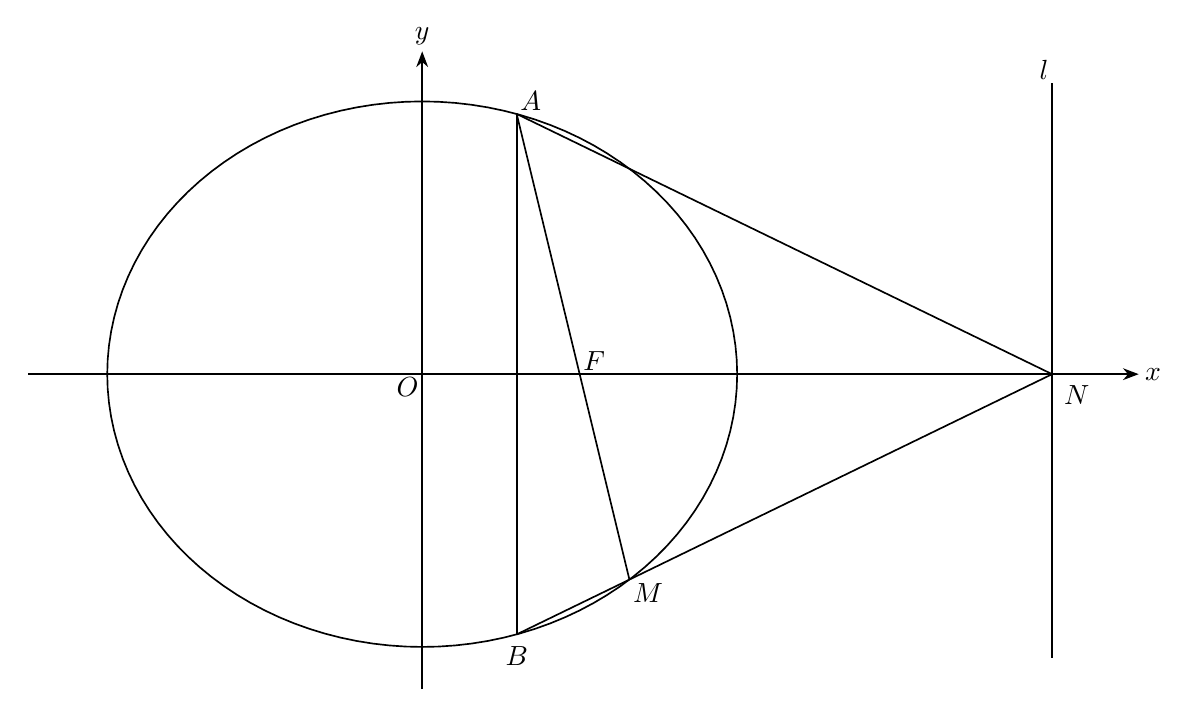
\begin{tikzpicture}[x=2cm,y=2cm,line width=.6pt,font=\normalsize,>=Stealth]
  % axes
  \draw[->] (-2.5,0) -- (4.55,0) node[right,inner sep=0pt,xshift=2pt] {$x$};
  \draw[->] (0,-2.0) -- (0,2.05) node[above,inner sep=0pt,yshift=2pt] {$y$};
  % ellipse x^2/4 + y^2/3 = 1
  \draw plot[domain=0:360,samples=121,variable=\t] ({2*cos(\t)},{1.73205081*sin(\t)});
  % key points
  \coordinate (A) at (0.6,1.65227124);
  \coordinate (B) at (0.6,-1.65227124);
  \coordinate (F) at (1,0);
  \coordinate (N) at (4,0);
  \coordinate (M) at (1.31578947,-1.30442430);
  % vertical chord AB
  \draw (A) -- (B);
  % line AFM and line BMN and segment AN
  \draw (A) -- (M);
  \draw (B) -- (N);
  \draw (A) -- (N);
  % directrix / line l: x = 4
  \draw (4,-1.8) -- (4,1.85);
  % labels
  \node[above right=1pt,inner sep=0pt] at (A) {$A$};
  \node[below=4pt,inner sep=0pt] at (B) {$B$};
  \node[below right=1pt,inner sep=0pt] at (M) {$M$};
  \node[above right=1pt,inner sep=0pt] at (F) {$F$};
  \node[below right=4pt,inner sep=0pt] at (N) {$N$};
  \node[above left=1pt,inner sep=0pt] at (4,1.85) {$l$};
  \node[below left=1pt,inner sep=0pt] at (0,0) {$O$};
\end{tikzpicture}
